% XeLaTeX can use any Mac OS X font. See the setromanfont command below.
% Input to XeLaTeX is full Unicode, so Unicode characters can be typed directly into the source.

% The next lines tell TeXShop to typeset with xelatex, and to open and save the source with Unicode encoding.

%!TEX TS-program = XeLaTeX
%!TEX encoding = UTF-8 Unicode

\documentclass[11pt]{scrreprt}

\usepackage{flupstyleutfxelatex}

%\usepackage{geometry}                % See geometry.pdf to learn the layout options. There are lots.
\geometry{a4paper}                   % ... or a4paper or a5paper or ... 
%\geometry{landscape}                % Activate for for rotated page geometry
%\usepackage[parfill]{parskip}    % Activate to begin paragraphs with an empty line rather than an indent
\usepackage{graphicx}
\usepackage{amssymb}

% Will Robertson's fontspec.sty can be used to simplify font choices.
% To experiment, open /Applications/Font Book to examine the fonts provided on Mac OS X,
% and change "Hoefler Text" to any of these choices.

\usepackage[frenchb]{babel}

\usepackage{fontspec,xltxtra,xunicode}
%\usepackage{fontspec,xunicode,luatextra}

%\defaultfontfeatures{Mapping=tex-text}
\defaultfontfeatures{Ligatures=TeX}

%\setromanfont[Mapping=tex-text]{Garaline Regular}
%\setromanfont{Linux Libertine O}
%\setsansfont[Scale=MatchLowercase,Mapping=tex-text]{Gill Sans}
%\setmonofont[Scale=MatchLowercase]{Andale Mono}

%\defaultfontfeatures{Mapping=tex-text, Fractions=On} 
%\defaultfontfeatures{Mapping=tex-text} 
%\setromanfont [Ligatures={Common}, Numbers={OldStyle}, Variant=02]{Linux Libertine O} 
%\setromanfont [Ligatures={Common}, Numbers={OldStyle}, Variant=01]{Linux Libertine O}
\setromanfont{Linux Libertine O}
\setsansfont{Linux Biolinum O}

\usepackage{polyglossia}
\setdefaultlanguage{french}

\usepackage{tikz}
%\usepackage{fetatolatex}
\usepackage{fancyhdr}
\usepackage{lilyglyphs}
\newcommand{\coda}{\lilyGlyph[scale=1.4, raise=0.5]{scripts.coda}}
\newcommand{\segno}{\lilyGlyph[scale=1.4, raise=0.5]{scripts.segno}}
\newcommand{\fermatalong}{\hspace{1ex}\lilyGlyph[scale=1.4, raise=0.5]{scripts.ulongfermata}}
\newcommand*{\wholeNote}[1][]{%
	\setkeys{lilyDesignOptions}{scale=1.3,raise=0.4}%
	\lilyPrint[#1]{\hspace*{0.25ex}\lilyGetGlyph{noteheads.s0}}%
}


\usepackage{microtype}
\usepackage{multirow}
%\usepackage[french=guillemets*]{csquotes}
%\MakeOuterQuote{"}
\frenchspacing
\usepackage{hyperref}
%\newcommand{\ieme}{\textsuperscript{ieme}}
%\newcommand{\iere}{\textsuperscript{iere}}
\setlength{\parindent}{0pt} %Supprime l'indentation en début de paragraphe
\usepackage{makeidx}
\makeindex
\FrenchFootnotes
%\usepackage{libertineotf}

% taking care of orphans/widows 
\widowpenalty=10000 
\clubpenalty=10000 
\raggedbottom
\sloppy

\title{Brief Article}
\author{The Author}
%\date{}                                           % Activate to display a given date or no date





%%Classe de document
%\documentclass[11pt,a4paper]{scrreprt}
%%!TEX encoding = UTF-8 Unicode
%
%%%%%%%%%%%%%% Les paquetages inclus maintenant dans les style bredele: %%%%%%%%%%%%%
%%Francisation
%%\usepackage [latin1] {inputenc} 
%%\usepackage [LGR,T1] {fontenc} % Saisie fran??ais + grec
%%\usepackage [greek, frenchb] {babel}
%%\usepackage[babel]{csquotes}
%
%%R?©glages g?©n?©rauxw
%%\usepackage{graphicx}
%%\usepackage{textcomp} %Acc??s aux symboles Euro, etc.
%%\usepackage[style=authortitle,hyperref]{biblatex}
%%\usepackage{fancyhdr}
%%\FrenchFootnotes
%%\fancyhead[LE,RO]{\thepage}
%%\fancyhead[CE]{\scshape \leftmark}
%
%%%%%%%%%%%%%% Les paquetages divers dªsactivªs: %%%%%%%%%%%%%
%%\makeatletter
%%\DeclareGraphicsExtensions{.pdf, .jpg, .tif, .gif}
%%\AddThinSpaceBeforeFootnotes
%%\fancyhead[CO]{\scshape \rightmark}
%%fancyfoot[CO]{}
%%\pagestyle{headings}
%%\pagestyle{plain}
%% En-tete
%%\lhead{}        \chead{En-tte}        \rhead{}
%\usepackage{tikz}
%\usepackage{flupstyleutf}
%\bibliography{flup}
%\usepackage{harmony}
%\usepackage{makeidx}
%\usepackage{pdfpages}
%\usepackage[colorlinks=black]{hyperref}
%%\usepackage{ae}
%\usepackage{musixtex}
%\setlength{\parindent}{0pt} %Supprime l'indentation en début de paragraphe
%\pagestyle{fancy}
%\usepackage[bitstream-charter]{mathdesign}
%%\usepackage{libertine}
%\renewcommand*\oldstylenums[1]{{\fontfamily{fxlj}\selectfont #1}}
%\usepackage{multirow}
%\makeindex
%
%\usepackage{tikz}
%\usetikzlibrary{arrows}
\begin{document}
%--------------------------PAGE DE GARDE-------------------
%----------------------------------------------------------------------
\thispagestyle{empty}
\pagenumbering{roman}
\begin{center}
\begin{LARGE}
Académie des Arts de Bruxelles-Ville
\end{LARGE}
\end{center}

\begin{center}
\begin{LARGE}
\textbf{Cours de formation musicale}
\end{LARGE}
\end{center}

\begin{center}
\vspace{5cm}
\noindent\rule{\textwidth}{0.5mm}
\begin{huge}
\textbf{Aide-mémoire de théorie \\
\vspace{2 cm}
 Formation 1 à 3}
\end{huge}
\noindent\rule{\textwidth}{0.5mm}
\end{center}

%------------------------------------INTRODUCTION--------------------
%------------------------------------------------------------------------------
%\clearpage
%\thispagestyle{empty}
%%\addcontentsline{toc}{chapter}{\numberline{}Remerciements}
%%\chapter*{Remerciements}
%\begin{vcenterpage}
%
%
%\paragraph{À l'attention des parents}
%\paragraph{}
%Ce petit aide-mémoire reprend les différentes notions de théorie correspondant à chaque degré de formation musicale à l'académie. Chaque professeur expliquera ces notions à sa manière devant les élèves, mais les pages qui suivent permettent de retrouver rapidement les différents chapitres vus pendant l'année, de façon résumée mais néanmoins précise.
%
%
%\end{vcenterpage}
%--------------------------TDM ETC------------ ------------------------
%------------------------------------------------------------------------------
\newpage
\selectlanguage{french}
\pagenumbering{roman}
\fancyfoot[CO]{\thepage}%ajouter CE si a marche pas
\renewcommand{\contentsname}{Sommaire}
\tableofcontents
%\sommaire
%\listoffigures
\cleardoublepage
%--------------------------CHAPITRES------------ ----------------
%------------------------------------------------------------------------------
%!TEX root = theorie_solfege_Bxl.tex
\clearpage
\pagenumbering{arabic}
\lhead{Aide-mémoire de théorie}
\rhead{Formation 1}
\fancyfoot[CO]{\thepage}%ajouter CE si ça marche pas

\chapter{Les valeurs de notes et de silences}
\section{Les valeurs de notes}
Le dessin des notes est constitué de 3 parties:
\begin{itemize}
\item la tête de la note (noire, blanche, ronde)
\item la hampe\index{hampe} (la barre sur le côté. À droite vers le haut, ou à gauche vers le bas)
\item le crochet\index{crochet} (quand les notes sont accrochées, on parle de \emph{ligature}\index{ligature})
\end{itemize}

Voici les valeurs rythmiques les plus courantes:
%\begin{center}
%\includegraphics{exemples/diagrammenotes}\label{tableaunotes}
%\end{center}


\begin{center}\label{tableaunotes} 

\begin{tikzpicture}
[level distance=15mm,
level 1/.style={sibling distance=90mm}, 
level 2/.style={sibling distance=40mm}, 
level 3/.style={sibling distance=20mm},
level 4/.style={sibling distance=12mm},
level 5/.style={sibling distance=5mm}]

\node {\wholeNote} child {node {\halfNote}
child {node {\crotchet} child {node {\quaver} child {node {\semiquaver}} child {node {\semiquaver}} } child {node {\quaver} child {node {\semiquaver}} child {node {\semiquaver}} } 
} child {node {\crotchet}
child {node {\quaver} child {node {\semiquaver}} child {node {\semiquaver}} } child {node {\quaver} child {node {\semiquaver}} child {node {\semiquaver}} }
}
} 
child {node {\halfNote}
child {node {\crotchet} child {node {\quaver} child {node {\semiquaver}} child {node {\semiquaver}} } child {node{\quaver} child {node {\semiquaver}} child {node {\semiquaver}} }
}
child {node {\crotchet} child {node{\quaver} child {node {\semiquaver}} child {node {\semiquaver}} } child{node{\quaver} child {node {\semiquaver}} child {node {\semiquaver}} }   }
};
\end{tikzpicture}
\end{center}



\section[La noire]{La noire \crotchet}\index{noire}
La noire est la valeur rythmique la plus simple; elle correspond souvent à une pulsation et à un temps (dans les mesures \lilyTimeSignature{2}{4}, \lilyTimeSignature {3}{4} ou \lilyTimeSignature{4}{4}).
\section[La blanche]{La blanche \halfNote}\index{blanche}
Elle vaut 2 noires. Elle se poursuit donc sur 2 noires entières, jusqu'au bout de la 2\ieme { }(juste avant le début de la pulsation suivante)
\section[La ronde]{La ronde \wholeNote}\index{ronde}
La ronde vaut 4 noires ou 2 blanches. Elle sert également à calculer les chiffres de mesure.
\section[La croche]{La croche \quaver}\index{croche}
Une croche seule vaut la moitié d'une noire. Pour obtenir la même durée qu'une noire, il faut donc 2 croches. Comme leur nom l'indique, ces notes peuvent s'accrocher et s'écrire ainsi: \twoBeamedQuavers{}
Mais, même accrochées, il s'agit toujours bien de 2 croches.
\section[La double croche]{La double croche \semiquaver}\index{double croche}
Une double croche seule vaut le quart d'une noire. Pour obtenir la même durée qu'une noire, il en faut donc 4. Il en faudra 2 pour obtenir la durée d'une croche. Comme les croches, ils peuvent s'accrocher. %Groupées par 4, elles s'écrivent ainsi: \Vier\SechBL\SechBL\SechBL

\section{Les valeurs de silences}
À chaque valeur de note correspond une valeur de silence:
\begin{itemize}
\item la pause\index{pause} \hspace{1ex}\wholeNoteRest{}\hspace{1ex} (sous la 4\ieme{} ligne) correspond à la ronde
\item demi-pause\index{demi-pause} \hspace{1ex}\halfNoteRest\hspace{1ex} (sur la 3\ieme{} ligne) correspond à la blanche
\item le soupir\index{soupir} \crotchetRest{} correspond à la noire
\item le demi-soupir\index{demi-soupir} \quaverRest{} correspond à la croche
\item le quart de soupir\index{quart de soupir} \semiquaverRest{} correspond à la double-croche .
\end{itemize}

La pause peut aussi être utilisée pour remplir une mesure de silence: elle prend alors la valeur de la mesure complète.
%\begin{center}
%\includegraphics{exemples/diagrammesilences}
%\end{center}

\begin{center}

\begin{tikzpicture} 
[level distance=15mm,
level 1/.style={sibling distance=90mm}, 
level 2/.style={sibling distance=40mm}, 
level 3/.style={sibling distance=20mm},
level 4/.style={sibling distance=12mm},
level 5/.style={sibling distance=5mm}]

\node {\wholeNoteRest} child {node {\halfNoteRest}
child {node {\crotchetRest} child {node {\quaverRest} child {node {\semiquaverRest}} child {node {\semiquaverRest}} } child {node {\quaverRest} child {node {\semiquaverRest}} child {node {\semiquaverRest}} } 
} child {node {\crotchetRest}
child {node {\quaverRest} child {node {\semiquaverRest}} child {node {\semiquaverRest}} } child {node {\quaverRest} child {node {\semiquaverRest}} child {node {\semiquaverRest}} }
}
} 
child {node {\halfNoteRest}
child {node {\crotchetRest} child {node {\quaverRest} child {node {\semiquaverRest}} child {node {\semiquaverRest}} } child {node{\quaverRest} child {node {\semiquaverRest}} child {node {\semiquaverRest}} }
}
child {node {\crotchetRest} child {node{\quaverRest} child {node {\semiquaverRest}} child {node {\semiquaverRest}} } child{node{\quaverRest} child {node {\semiquaverRest}} child {node {\semiquaverRest}} }   }
};
\end{tikzpicture}
\end{center}



\section{Le point d'augmentation}
Le point\index{point} prolonge la note de la moitié de sa valeur. Il se place à droite de la note. 

Exemples:
\begin{description}
\item \halfNoteDotted{} = \halfNote { } + \crotchet
\item \crotchetDotted{} = \crotchet { } + \quaver
\end{description}
S'il y en a un deuxième, il vaut la moitié du premier point: \halfNoteDottedDouble{} = \halfNote { } + \crotchet { } + \quaver{} 

On peut aussi ajouter un point aux silences, mais on préfère généralement écrire 2 silences séparés ( \crotchetRest{} \quaverRest{} ) plutôt qu'un silence pointé ( \crotchetRestDotted{} ).

\section{La liaison rythmique}\index{liaison rythmique}
Les valeurs de 2 notes identiques liées s'additionnent pour former une valeur unique. Dans ces 2 exemples, la note \emph{mi} a la même durée.
\begin{flushleft}
\includegraphics{exemples/liaisonrythmique}  \hspace{2 cm}\includegraphics{exemples/liaisonrythmique2} 
\end{flushleft}

%!TEX root = theorie_solfege_Bxl.tex
\chapter{La mesure}\index{mesure}

\section{La pulsation et le temps}\index{pulsation}
\subsubsection{La pulsation}
La pulsation est un battement régulier, un peu comme les battements de c\oe{}ur. Elle marque le début de chaque temps. La succession des pulsations indique la durée des temps ainsi que le tempo.
\subsubsection{Le temps}\index{temps}
Le temps est la durée entre une pulsation et la suivante.
\subsubsection{La tempo}\index{tempo}
Le tempo correspond à la vitesse à laquelle les pulsations se suivent.

\section{La battue de mesure}\index{battue}
Le mouvement est très important: il nous permet de savoir et de sentir sur quel temps de la mesure nous nous trouvons. Dans un orchestre, il permet aux musiciens de savoir quand il vont devoir commencer à jouer. Le premier temps est \emph{toujours} vers le bas.

\subsubsection{Mesure à 2 temps}
\begin{tikzpicture}
\draw [thick, latex-] (0,0) -- (0,2) node [below=2cm]{1}; 
\draw [thick, -latex] (1,0) -- (1,2) node [below=2cm]{2}; 
\end{tikzpicture}

\subsubsection{Mesure à 3 temps}
\begin{tikzpicture}
\draw [thick, latex-] (0,0) -- (0,1.8) node [below=1.8cm]{1}; 
\draw [thick, -latex] (0.2,0) -- (2,0) node [right=2pt]{2}; 
\draw [thick, -latex] (2,0.2) -- (0,2) node [above=2pt]{3}; 
\end{tikzpicture}

\subsubsection{Mesure à 4 temps}
\begin{tikzpicture}
\draw [thick, latex-] (2,0) -- (2,2) node [below=1.9cm]{1}; 
\draw [thick, -latex] (1.8,0) -- (0,0) node [left=2pt]{2}; 
\draw [thick, -latex] (0,-0.4) -- (4,-0.4) node [right=1pt]{3}; 
\draw [thick, -latex] (4,-0.2) -- (2.2,2) node [above=2pt]{4}; 
\end{tikzpicture}

Il existe d'autres mouvements de mesures (6 temps lents, 5 temps), mais on les utilise rarement.

\section{Mesures binaires et ternaires}
\subsection{Mesures binaires}\index{binaire}
Les mesures binaires sont les mesures dont les temps sont divisibles par 2: \lilyTimeSignature{2}{4}, \lilyTimeSignature{3}{4}, \lilyTimeSignature{4}{4}, etc. On les appelle aussi \emph{mesures simples}.\index{mesure simple}

\subsection{Mesures ternaires}\index{ternaire}
Les mesures ternaires sont les mesures dont les temps sont divisibles par 3: \lilyTimeSignature{6}{8}, \lilyTimeSignature{9}{8}, \lilyTimeSignature{12}{8}, etc. Même si \lilyTimeSignature{6}{8} indique une mesure de 6 croches, il ne s'agit généralement pas d'une mesure à 6 temps (sauf en tempo lent), mais d'une mesure à 2 temps, chaque temps valant 3 croches (ou une noire pointée). On les appelle aussi \emph{mesures composées}.\index{mesure composée}


%\subsubsection{Mesure à 6 temps}
%\begin{tikzpicture}
%\draw [thick, latex-] (2,0) -- (2,2) node [below=1.9cm, left=2pt]{1}; 
%\draw[thick, ->] (2.1,0) arc (180:0:8pt) node [below=-0.7cm]{2};
%\draw[thick, ->] (2.9,0) arc (180:0:8pt) node [below=-0.7cm]{3};
%\draw [thick, -latex] (3.6,-0.2) -- (0,-0.2) node [left=2pt]{4}; 
%\draw [thick, -latex] (0,-0.5) -- (4.5,-0.5) node [right=1pt]{5}; 
%\draw [thick, -latex] (4.5,-0.3) -- (2.2,2) node [above=2pt]{6}; 
%\end{tikzpicture}

%\subsubsection{Mesure à 5 temps}
%\begin{tikzpicture}
%\draw [thick, latex-] (2,0) -- (2,2) node [below=1.9cm, right=2pt]{1}; 
%\draw[thick, ->] (1.9,0) arc (0:180:8pt) node [below=-0.7cm]{2};
%\draw[thick, ->] (1.2,0) arc (0:180:8pt) node [below=-0.7cm]{3};
%\draw [thick, -latex] (0.5,-0.2) -- (4.5,-0.2) node [right=1pt]{4}; 
%\draw [thick, -latex] (4.5,0) -- (2.2,2) node [above=2pt]{5}; 
%\end{tikzpicture}

\section{La barre de reprise}
Pour indiquer qu'il faut répéter une ou plusieurs mesures, on utilise parfois des barres de reprises. Toutes les mesures comprise entre 2 barres de reprises (ou entre le début et une barre de reprise) doivent être rejouées. Cela permet de ne pas devoir ré-écrire un passage complet et d'économiser de la place.

\includegraphics{exemples/reprise}

\section{Les chiffres de mesure}\index{chiffres de mesure}
Les chiffres de mesure comptent toujours 2 nombres:
\begin{itemize}
\item le premier (au-dessus) indique le nombre de pulsations par mesure
\item le deuxième (en-dessous) indique la valeur de chaque pulsation
\end{itemize}


Pour savoir à quelle valeur correspond le deuxième nombre, on divise une ronde comme dans le tableau des valeurs de notes (page \pageref{tableaunotes}):
\begin{itemize}
\item 1 = une ronde
\item 2 = une blanche (la moitié d'une ronde)
\item 4 = une noire (le quart d'une ronde)
\item 8 = une croche (le huitième d'une ronde)
\end{itemize}
Une mesure \lilyTimeSignature{2}{4} indique donc 2 temps par mesure, chaque temps valant une noire. Une mesure \lilyTimeSignature{2}{2} indiquera aussi 2 temps par mesure, mais chaque temps vaudra alors une blanche.


%!TEX root = theorie_solfege_Bxl.tex
\chapter{Les intervalles}

Un intervalle\index{intervalle} est la distance entre 2 notes. Il y a plusieurs façons de la calculer:

\begin{enumerate}
\item compter le nombre de notes différentes de l'intervalle
\item calculer les tons et les demi-tons
\end{enumerate}

\section{Compter les notes de l'intervalle}
Il suffit de compter - sur les doigts, par exemple - le nombre de notes, de la première à la dernière, en suivant l'ordre des notes. Si l'intervalle descend, on compte en utilisant l'ordre descendant.

Chaque nombre de notes correspond à un nom (le nom de l'intervalle):
%\begin{multicols}{2}
\begin{description}
\item 2 notes: seconde\index{seconde} 
\item \includegraphics[width=3cm]{exemples/secondemaj.pdf}
\item 3 notes: tierce\index{tierce}
\item \includegraphics[width=3cm]{exemples/tiercemaj.pdf}
\item 4 notes: quarte\index{quarte}
\item \includegraphics[width=3cm]{exemples/quarteaug.pdf}
\item 5 notes: quinte\index{quinte}
\item \includegraphics[width=3cm]{exemples/quintejuste.pdf}
%\columnbreak
\item 6 notes: sixte\index{sixte}
\item \includegraphics[width=3cm]{exemples/sixtemaj.pdf}
\item 7 notes: septième\index{septième}
\item \includegraphics[width=3cm]{exemples/septmaj.pdf}
\item 8 notes: octave\index{octave}
\item \includegraphics[width=3cm]{exemples/octavejuste.pdf}
\end{description}
%\end{multicols}

Comme cette mesure de l'intervalle n'est pas très précise (un nom d'intervalle peut avoir plusieurs tailles différentes), on compte les tons et demi-tons de l'intervalle pour être plus précis.

\section{Compter les tons et demi-tons}\index{ton}\index{demi-ton}
Les tons et demi-tons permettent de calculer de façon précise la taille d'un intervalle. Pour les repérer facilement, on utilise le clavier du piano:

\begin{itemize}
\item quand deux touches sont séparées par une autre touche, la distance entre elles est d'un ton
\item quand il n'y a aucune touche entre elles, la distance entre elles est d'un demi-ton
\end{itemize}
\begin{center}
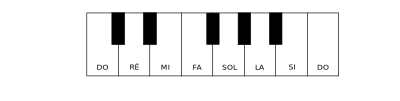
\includegraphics[width=12cm]{exemples/clavier.pdf}\index{clavier}
\end{center}

%\begin{center}
%\includegraphics{exemples/intervallesF1.pdf}\index{intervalle}
%\end{center}

\chapter{Les intervalles}\index{intervalle}
\section{Intervalles}
Un intervalle est la distance entre deux notes. Elle se calcule de plusieurs façons:
\begin{description}
\item[nom de l'intervalle:] en fonction du nombre de notes de l'intervalle (voir plus bas) 
\item[contenance:]\index{contenance} le nombre de tons et demi-tons contenus de l'intervalle
\item[qualification:]\index{qualification} la combinaison des 2 précédents, qui qualifie l'intervalle de majeur, mineur, juste, augmenté ou diminué
\end{description}

\section{Tons et demi-tons}
Le ton est constitué de l'addition d'un demi-ton diatonique et d'un demi-ton chromatique.
\subsubsection{Le demi-ton diatonique}\index{diatonique}
C'est le demi-ton situé entre deux notes de noms différents. Exemples: mi -- fa ou do \sharp{} -- ré. Il compte 4 commas\footnote{Le comma est une subdivision du ton. Par convention et simplification, on considère que le ton en compte~9.}.
\subsubsection{Le demi-ton chromatique}\index{chromatique}
C'est le demi-ton situé entre 2 notes de nom identique. Il compte 5 commas. Exemple: si -- si \flat

\section{Calcul de l'intervalle}
%Par convention et de façon à maintenir la logique tonale, on maintient la différence écrite et logique entre ces deux demi-tons, malgré l'absence de différence sonore.

\subsection{Les noms d'intervalles}
\begin{description}
%\item [1 note:] prime
\item [2 notes:] seconde
\item [3 notes:] tierce
\item [4 notes:] quarte
\item [5 notes:] quinte
\item [6 notes:] sixte
\item [7 notes:] septième
\item [8 notes:] octave
\end{description}
Il existe évidemment des intervalles plus grands; leur nom est très facile à retenir: neuvième (9 notes), dixième (10 notes), onzième (11 notes) etc.\\

\textbf{Rappel}: on compte toujours la note de départ, celle d'arrivée et toutes celles qui sont située entre les 2.
\subsection{La contenance}\index{contenance}
Il s'agit de la quantité de tons et demi-tons contenue dans un intervalle. Attention aux additions de demi-tons!

\subsection{La qualification}\index{qualification}
Il s'agit d'un qualificatif attribué à chaque intervalle, en fonction de son nom et de sa contenance. Il n'existe qu'un seul intervalle portant le même nom et ayant la même contenance.

Certains intervalles peuvent être \emph{majeurs} (M) ou \emph{mineurs} (m). D'autres ne peuvent pas l'être mais pourront être \emph{justes}. Tous les intervalles peuvent également être augmentés et diminués.\\


En résumé:
\begin{enumerate}
\item quartes, quintes, octaves peuvent être justes, augmentées, diminuées
\item secondes, tierces, sixtes, septièmes peuvent être majeures, mineures, augmentées, diminuées.
\end{enumerate}

\subsection{Le renversement}\index{renversement}
Un intervalle peut-être renversé: on fait passer une des 2 notes par-dessus ou par-dessous l'autre, sans changer le nom des notes. La qualification d'un intervalle est inversée en cas de renversement. Exemple: en renversant une sixte mineure, on obtiendra une tierce majeure.

\centerline{\includegraphics[width=5cm]{exemples/renversement}}

%\subsection{Le redoublement}\index{redoublement}
%Un intervalle redoublé est un intervalle plus grand qu'une octave. Sa qualification se calcule en ne tenant compte que de l'intervalle dépassant l'octave juste. Exemple: une neuvième de 6 tons et $\frac2 2$ aura la même qualification qu'une seconde de 1 ton.\\

\pagebreak
Voici un tableau récapitulatif des contenances et qualifications d'intervalles de base.
\begin{center}
\begin{tabular}[width=15cm]{|c|c|c|c|c|c|}
\hline
Nom & diminuée & mineure & juste & majeure & augmentée\\
\hline
&&&&&\\
\multirow{2}{*} {seconde} &&\includegraphics[width= 2.35cm]{exemples/secondemin}&&\includegraphics[width= 2.35cm]{exemples/secondemaj}&\\
& & $\frac 1 2$ ton d & & 1 ton & \\ 
&&&&&\\ \hline
&&&&&\\
\multirow{2}{*} {tierce} &&\includegraphics[width= 2.35cm]{exemples/tiercemin}&&\includegraphics[width= 2.35cm]{exemples/tiercemaj}&\\
& & 1 ton $\frac1 2$ d & & 2 tons & \\
&&&&&\\ \hline
&&&&&\\
\multirow{2}{*} {quarte} && &\includegraphics[width= 2.35cm]{exemples/quartejuste}&&\includegraphics[width= 2.35cm]{exemples/quarteaug}\\
& & & 2 tons $\frac1 2$ d & & 3 tons\\
&&&&&\\ \hline
&&&&&\\
\multirow{2}{*} {quinte} &\includegraphics[width= 2.35cm]{exemples/quintedim}& &\includegraphics[width= 2.35cm]{exemples/quintejuste}&&\\
& 2 tons $\frac2 2$ d & & 3 tons $\frac1 2$ d & & \\
&&&&&\\ \hline
&&&&&\\
\multirow{2}{*} {sixte} &&\includegraphics[width= 2.35cm]{exemples/sixtemin}&&\includegraphics[width= 2.35cm]{exemples/sixtemaj}&\\
& & 3 tons $\frac2 2$ d & & 4 tons $\frac1 2$ d & \\
&&&&&\\ \hline
&&&&&\\
\multirow{2}{*} {septième} &&\includegraphics[width= 2.35cm]{exemples/septmin}&&\includegraphics[width= 2.35cm]{exemples/septmaj}&\\
& & 4 tons $\frac2 2$ d& & 5 tons $\frac12$ d & \\
&&&&&\\ \hline
&&&&&\\
\multirow{2}{*} {octave} && &\includegraphics[width= 2.35cm]{exemples/octavejuste}&&\\
&  & & 5 tons $\frac2 2$ d & & \\
&&&&&\\
\hline
\end{tabular}
\end{center}



\section{Les altérations}\index{altération}
Les altérations servent à modifier la hauteur de notes, soit vers le haut (plus aiguë), soit vers le bas (plus grave):
\begin{itemize}
\item le dièse \sharp \index{dièse}\index{\sharp} sert à monter une note d'un demi-ton
\item le bémol \flat \index{bémol}\index{\flat} sert à descendre une note d'un demi-ton.
\end{itemize}
Le bécarre \natural\index{bécarre}\index{\natural} sert à annuler l'effet d'un \sharp{} ou d'un \flat. 

Les \sharp{} et \flat{} sont donc souvent des touches noires (mais pas toujours).
%!TEX root = theorie_solfege_Bxl.tex
\chapter{Gammes, tonalités}
\section{Gammes}\index{gamme}
Une gamme est une suite d'intervalle. Il existe de nombreuses gammes et le nombre de notes qu'elles contiennent n'est pas toujours le même. Cependant, il existe 2 gammes très connues (gamme majeure et gamme mineure) et elles comptent chacune 8 notes, donc 7 différentes (la 8\ieme{} porte le même nom que la première).
\subsection{La gamme majeure}\index{gamme majeure}
C'est la gamme la plus connue. Elle est fabriqué à partir d'une suite de tons et de demi-tons dans cet ordre:
\begin{center}
\fbox{1t - 1t - $\frac 1 2$ t - 1t - 1t - 1t - $\frac 1 2$ t}
\end{center}
\subsubsection{Do Majeur}

Voici l'exemple de Do Majeur.\index{do majeur}
\begin{center}
\includegraphics{exemples/gamme_maj.pdf}
\end{center}

Il existe beaucoup d'autres gammes majeures. Pour respecter l'ordre des tons et demi-tons dans la gamme, il faut monter ou abaisser certaines notes, en utilisant des \sharp{} ou \flat. Voici 2 exemples:
\subsubsection{Sol Majeur}\index{sol majeur}
\begin{center}
\includegraphics{exemples/sol_maj.pdf}
\end{center}

\subsubsection{Fa Majeur}\index{fa majeur}
\begin{center}
\includegraphics{exemples/fa_maj.pdf}
\end{center}

\subsection{La gamme mineure}
La gamme mineure possède plusieurs formes couramment utilisées. Toutes sont malgré tout basées sur la gamme mineure \emph{antique}, qui est la seule à correspondre à son armure.

\subsubsection{Gamme mineure antique\label{min_ant}}\index{gamme mineure antique}
\begin{center}
\includegraphics{exemples/gamme_min_ant.pdf}
\end{center}

Elle est construite sur le schéma suivant: 
\begin{center}
\fbox{1t - $\frac 1 2$ t - 1t - 1t - $\frac 1 2$ t - 1t - 1t}
\end{center}
Le 7\ieme{} degré est ici appelé \emph{sous-tonique}\index{sous-tonique} et non \emph{sensible}, vu qu'il y a 1 ton entre cette note et la tonique.

\subsubsection{Gamme mineure harmonique}\index{gamme mineure harmonique}
\begin{center}
\includegraphics{exemples/gamme_min_har.pdf}
\end{center}

Pour palier à l'absence de sensible, cette gamme présente un 7\ieme{} degré haussé, devenant ainsi une sensible. Par contre, l'intervalle VI - VII d'1 ton $\frac1 2$ (seconde augmenté) rend cette gamme mélodique. Son nom  \og harmonique \fg{} indique d'ailleurs qu'elle est utilisé pour constituer l'harmonie et les accords d'une musique.

Elle est construite sur le schéma suivant: 
\begin{center}
\fbox{1t - $\frac 1 2$ t - 1t - 1t - $\frac 1 2$ t - 1t $\frac 1 2$ - $\frac 1 2$ t}
\end{center}

\subsubsection{Gamme mineure mélodique}\index{gamme mineure mélodique}
Tout en conservant la sensible introduite dans la gamme mineure harmonique, elle rétablit l'intervalle VI - VII d'1 ton, rendant la gamme beaucoup plus adaptée à l'écriture mélodique. Cette gamme, contrairement aux autres possède une forme descendante différente de la forme ascendante (montante), et qui est similaire à la gamme antique.

Elle est construite sur le schéma suivant: 
\begin{center}
\fbox{1t - $\frac 1 2$ t - 1t - 1t - 1t - 1t  - $\frac 1 2$ t}
\end{center}
\begin{center}
\includegraphics{exemples/gamme_min_mel.pdf}
\end{center}
%D'autres gammes sont souvent associées aux gammes mineures (gamme mixte, gamme bohémienne, gamme  orientale) mais il est plus logique de les considérer comme des modes à part entière\footnote{L'aberration consistant à considérer la gamme mixte comme gamme mineure -- alors que son accord parfait est majeur -- est un exemple parmi d'autres.}.

%Les autres modes ont malgré tout gardé une certaine importance, variable selon les époques et les lieux (musique populaire, jazz, musiques du monde etc.).

\subsection{L'accord parfait}\index{accord parfait}
L'accord parfait d'une gamme est composé de la 1\iere{} (tonique), la 3\ieme{} (médiante) et la 5\ieme{} (dominante) note d'une gamme. Jouées l'une après l'autre, ces notes forment un arpège\index{arpège}.


\section{Degrés}\index{degrés}
Chaque note dans la gamme porte un nom, en fonction de sa place. On numérote les notes de la gamme en utilisant les chiffres romains.
\begin{itemize}
\item la première (I) s'appelle \textbf{tonique}\index{tonique}
\item la deuxième (II) s'appelle \textbf{sus-tonique}\index{sus-tonique}
\item la troisième (III) s'appelle \textbf{médiante}\index{médiante}
\item la quatrième (IV) s'appelle \textbf{sous-dominante}\index{sous-dominante}
\item la cinquième (V) s'appelle \textbf{dominante}\index{dominante}
\item la sixième(VI) s'appelle \textbf{sus-dominante}\index{sus-dominante}
\item la septième (VII) s'appelle \textbf{sensible}\index{sensible}
\end{itemize}
La huitième note (VIII) est la même que la première.

Les plus importants à retenir sont la tonique, la dominante et la sensible.

En mineur antique (voir \ref{min_ant} page \pageref{min_ant}), la septième note de la gamme porte le nom de sous-tonique, étant donné qu'il y a un ton au lieu d'$\frac1 2$ entre cette dernière et la tonique. Les degrés de la gamme se notent de chiffres romains.

\section{Armures}
Les altérations présentes à l'armure se présentent toujours dans un ordre précis.
\subsubsection{Ordre des dièses}\index{ordre des dièses}
FA DO SOL RÉ LA MI SI
\subsubsection{Ordre des bémols}\index{ordre des bémols}
SI MI LA RÉ SOL DO FA
\\
\\
Cette armure permet de déterminer la tonalité majeure ou mineure présente dans une partition. À chaque armure correspondent 2 tonalités: une majeure, l'autre mineure. Par facilité, on calcule d'abord la possibilité majeure, avant de calculer la relative mineure.

\subsubsection{Tonalités en dièse}
Le dernier dièse présent à l'armure correspond à la sensible de la tonalité majeure. Il suffit donc de monter d'$\frac1 2$ ton diatonique à partir de cette note (qui est toujours un \sharp) pour obtenir le nom de la tonalité majeure.
\subsubsection{Tonalités en bémols}
La tonique correspond à l'avant-dernier \flat. Exception: Fa Majeur, dont l'armure est si \flat{} (puisqu'il n'y a pas dans ce cas d'avant-dernier \flat).

On peut imaginer les différentes tonalités formant une horloge: dans le sens des aiguilles d'une montre, on ajoute un \sharp; dans le sens contraire, on ajoute un \flat.
 %%%%%%%%%%CYCLE DES QUINTES%%%%%%%%%%%
\begin{center}
\begin{tikzpicture} [line cap=round,line width=1pt] 
\draw (0,0) circle (4.2cm);

\foreach \angle / \label in 
{0/{LA}, 30/{RÉ}, 60/{SOL}, 90/{DO}, 120/{FA}, 150/{SI \flat}, 180/{MI \flat},
210/{LA \flat}, 240/{DO \sharp{} - RÉ \flat}, 270/{FA \sharp{} - SOL \flat}, 300/{SI}, 330/{MI}}
{
\draw[line width=1pt] (\angle:4.0cm) -- (\angle:4.4cm); 
\draw (\angle:4.8cm) node{\label};
}
\foreach \angle / \label in 
{0/{3 \sharp}, 30/{2 \sharp}, 60/{1 \sharp}, 90/{$-$}, 120/{1 \flat}, 150/{2 \flat}, 180/{3 \flat},
210/{4 \flat}, 240/{7 \sharp{} - 5 \flat}, 270/{6 \sharp{} - 6 \flat}, 300/{5 \sharp{} - 7 \flat}, 330/{4 \sharp}}
{
\draw (\angle:3.6cm) node{\textsf{\label}};
}
\node (0,0){Gammes majeures};
\end{tikzpicture}
\end{center}

\begin{center}
\begin{tikzpicture} [line cap=round,line width=1pt] 
\draw (0,0) circle (4.2cm);

\foreach \angle / \label in 
{0/{fa \sharp}, 30/{si}, 60/{mi}, 90/{la}, 120/{ré}, 150/{sol}, 180/{do},
210/{fa}, 240/{la \sharp{} - si \flat}, 270/{ré \sharp{} - mi \flat}, 300/{sol \sharp}, 330/{do \sharp}}
{
\draw[line width=1pt] (\angle:4.0cm) -- (\angle:4.4cm); 
\draw (\angle:4.8cm) node{\label};
}
\foreach \angle / \label in 
{0/{3 \sharp}, 30/{2 \sharp}, 60/{1 \sharp}, 90/{$-$}, 120/{1 \flat}, 150/{2 \flat}, 180/{3 \flat},
210/{4 \flat}, 240/{7 \sharp{} - 5 \flat}, 270/{6 \sharp{} - 6 \flat}, 300/{5 \sharp{} - 7 \flat}, 330/{4 \sharp}}
{
\draw (\angle:3.6cm) node{\textsf{\label}};
}
\node (0,0){Gammes mineures};
\end{tikzpicture}
\end{center}

%!TEX root = theorie_solfege_Bxl.tex
\chapter{Termes musicaux}

Voici quelques termes musicaux ainsi que leur signification. Ces termes sont souvent en italien.

\section{Nuances}\index{nuances}
\begin{description}
\item \lilyDynamics{p} : doux, doucement (\emph{piano} en italien)
\item \lilyDynamics{f} : fort (\emph{forte} en italien)
\item \lilyDynamics{mf} : modérément fort (\emph{mezzo forte} en italien)
\item \lilyDynamics{mp}: modérément doux (\emph{mezzo piano} en italien)
\item Crescendo\index{crescendo} \crescHairpin{}: en augmentant l'intensité du son
\item Decrescendo\index{decrescendo} \decrescHairpin{}: en diminuant l'intensité du son
\end{description}

\section{Tempo et mesure}
\begin{description}
\item Lento: lent
\item Adagio: à l'aise
\item Andante: allant
\item Moderato: modéré
\item Allegro: rapide, joyeux
\item \lilyTimeC{}: mesure \lilyTimeSignature{4}{4}\index{\lilyTimeC{}}
\end{description}

\section{Divers}
\begin{description}
\item \fermata\index{point d'orgue} : point d'orgue. Prolonge une note ou un silence (durée au choix du musicien). Sur un silence, on parle de point d'arrêt. On peut aussi l'indiquer \fermatalong
\item Legato\index{legato} (lié): les notes sont jouées sans interruption du son entre elles.
\item \includegraphics{exemples/legato.pdf}
\item Staccato\index{staccato} (piqué): les notes sont jouées de façon courte. Le point est placé sous ou au-dessus de la note (à l'opposé de la hampe)
\item \includegraphics{exemples/staccato.pdf}
\item Anacrouse\index{anacrouse}: mesure incomplète au début d'un morceau de musique
\item Da capo (D. C.): reprendre au début 
\item Équisonance\index{equisonance@équisonance} ou enharmonie\index{enharmonie}: note de même son, mais de nom différent. Exemples: si~--~do~\flat{} ou fa~\sharp{} -- sol \flat.
\item Poco a poco: peu à peu, petit à petit
\item Tessiture\index{tessiture}: c'est l'ensemble des notes qu'un instrument peut jouer, du grave jusqu'à l'aigu. Elle permet de dire si un instrument est grave ou aigu.

\end{description}


\addcontentsline{toc}{chapter}{\numberline{}Index}
\printindex
\end{document}